\section{Implementation}\label{Sec_Imp}

\subsection{Communication (Abdul and/or Stefan)}

\subsection{Initialization procedure (Stephan and Stefan)}\label{Sec_Imp_Ini}

\subsubsection{Recording and filtering data (Stefan)}

\subsubsection{Analysing data (Stefan)}

\subsubsection[Selection of correct distance related to RSSI]{Selection of correct distance related to RSSI footnote{Stephan}}
In a first step the multiple occurring data points (see tbl.\ref{RSSI_Dis_data}) are divided into three groups (max, middle and min) where max means the maximal possible distance related to one RSSI and so on.\\ 
The measurements has shown that it is not trivial to define the correct distance related to most of the RSSI. The involved algorithm selects the correct distance out of the multiple possible solutions and is shown in fig. \ref{BestID}:\\
\begin{figure}[!htbp]
\centering
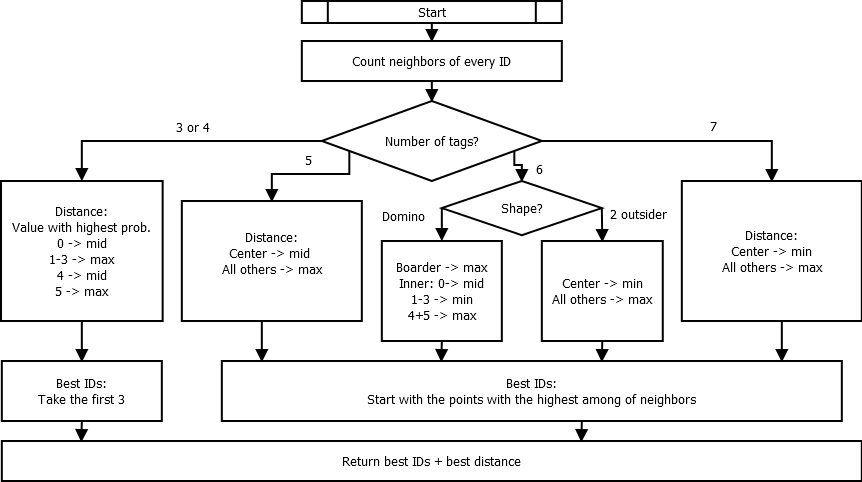
\includegraphics[width = 16cm]{Pictures/BestIDs}
\caption{Flow Chart: Selection of correct distance and most proper IDs}
\label{BestID}
\end{figure}\\
To distinguish between the multiple possible solution for one RSSI, the algorithm defines the shape of the pattern of tags based on the number of tags at each measurement and the number of the neighbours each tag has. At each measurement point are several numbers (4-7) of detected tags possible. The different shapes can be found in the tbl. \ref{ID_shapes}.\\
\begin{table}[!htbp]
\centering
\begin{tabular}{|c|c|c|c|c|c|}
\hline
\begin{tabular}[c]{@{}c@{}}Number of \\ detected tags \end{tabular}  & 4 & 5 & 6 (Domino) & 6 (2 alone)& 7 \\ \hline
Unique shapes        & 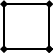
\includegraphics[width = 1.3cm]{Pictures/Shape1} & 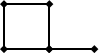
\includegraphics[width = 2.6cm]{Pictures/Shape2} &   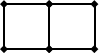
\includegraphics[width = 2.6cm]{Pictures/Shape3} & 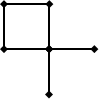
\includegraphics[width = 2.6cm]{Pictures/Shape4} & 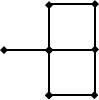
\includegraphics[width = 2.6cm]{Pictures/Shape5}\\ \hline
\end{tabular}
\caption{Possible shapes of pattern}
\label{ID_shapes}
\end{table}\\
Going back to the flow chart fig.\ref{BestID} the first step is to count the number of neighbours each tag has. With this information can the position of the tag in the pattern be detected. For example is a tag with 3 neighbours in a pattern of 5 tags the center of this pattern.\\
After the number of tags at each measurement point and the position of each tag are clear, the selecting of the correct distance will be performed based on the highest probability. To know the highest probabilities an analysis of measurements with emulated data has been done.\\
As an example are leading 4 detected tags to the fact that the position of the antenna should be very close to the center of this square. If in this case a RSSI of 4 is detected, the middle value (5.8 cm) will be taken. \\
Afterwards the most suitable three IDs will be selected, in case where more then three are detected. The algorithm takes at first the ID with the highest amount of neighbours, because these tags are close to the position of the antenna and have probably a value of 6 or 7 and are uniquely defined. In the case where several tags with the same number of tags, the first ID (number increasing) will be taken. \\
The return of the function is an array (2x3) with the indices of the chosen IDs and the correct distance. The correct distance will be indicated by the number 0,1 and 2. 0 means the maximal, 1 the middle and 2 the minimum possible value related to one RSSI. For example leads 
\[
\begin{bmatrix}
    3 & 2 & 4\\
    2 & 0 & 0 
\end{bmatrix} 
\]
to the choice of the maximal value of the RSSI of the fourth ID and the minimum value of the RSSI of the third and the fifth ID in the recorded array at this measurement point. \\

\subsubsection[Estimation of initial position and orientation]{Estimation of initial position and orientation \footnote{Stephan}}
As mentioned in sec.\ref{Sec_Imp_Ini}, the main idea to estimate the initial position is to find the intersection point, which lies in the middle of the measurement points.\\
To compute this position, the algorithm uses trilateration at every suitable measurement point to estimate its position. For trilatertion are three defined positions plus three radii necessary. Resulting from the last section, all these values are available.\\
\begin{figure}[!htbp]
\centering
\begin{minipage}{.5\textwidth}
\centering
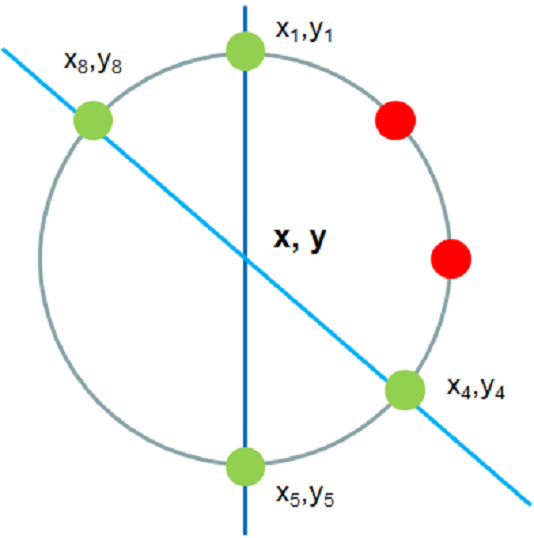
\includegraphics[width=5.5cm]{Pictures/Center_Rob} %
\caption{Computing the center of the robot}
\label{Center}
\end{minipage}%
\begin{minipage}{.5\textwidth}
\centering
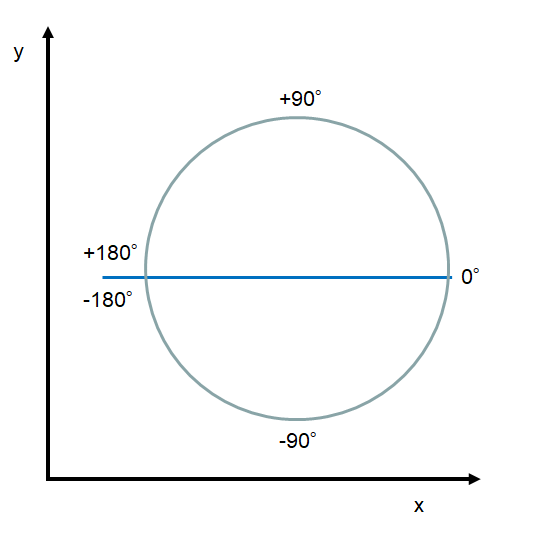
\includegraphics[width=5.5cm]{Pictures/Orientation} %
\caption{Orientation of robot in absolute angle}
\label{Angle}
\end{minipage}
\end{figure}\\
As follows from the fig.\ref{Center} shown above, the intersection point is found by computing two linear functions which go trough two corresponding points (blue lines). The center of the robot is then the intersection of those two linear functions and can be computed by the following equation:
\begin{align}
x = \dfrac{(x_1y_2-y_1x_2)(x_3-x_4)-(x_1-x_2)(x_3y_4-y_3x_4)}{(x_1-x_2)(y_3-y_4)-(y_1-y_2)(x_3-x_4)} \\
y = \dfrac{(x_1y_2-y_1x_2)(y_3-y_4)-(y_1-y_2)(x_3y_4-y_3x_4)}{(x_1-x_2)(y_3-y_4)-(y_1-y_2)(x_3-x_4)}
\end{align}
Theoretical are all eight measuring points suitable points (at least four IDs found). But for the case that the real measurements differ from the theory, the algorithm just needs four suitable points. \\
After the initial position as well as the positions of 4 measurement points are known, the algorithm computes the orientation based on those information. The relative angle between the center and the first measurement point will be computed with the arctan2 function. The orientation of the robot between -180$^\circ$ and +180$^\circ$ (see also fig.\ref{Angle}). \\
To compute the absolute angle, the angle of the measurement point has to be subtracted and 180$^\circ$ has to be added. This is caused by the fact that the antenna is placed on the back of the robot and the absolute orientation should be the direction of the front. After this computation, the initial position and orientation of the robot are known. \\

\subsection[Test setup]{Test setup\footnote{Stephan}}

\subsection[Results]{Results\footnote{Stephan}}

\subsection{Improvements}

